Whenever we deal with structures and the notion of a substructure is available to us, we can talk about densities of substructures within some larger structures. Even without formal definitions, the concept of density in permutations is so intuitive, that we can start thinking about it right away. It is easy to identify the ``problem'' of maximising the number of copies of a small fixed subpermutation in a larger permutation. Clearly, if we are trying to maximise the number of inversions (patterns $21$) in a permutation, we will not choose an increasing permutation for the job as it contains no inversions at all. We hint at the spectrum of densities for $123$ in Figure~\ref{fig:densities_spectrum}.

\begin{figure}[!ht]
\centering
\begin{subfigure}[t]{0.3\textwidth}
  \centering
  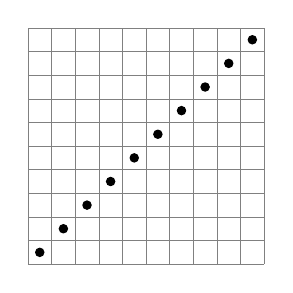
\begin{tikzpicture}[scale=0.3]
  \draw[gray, very thin] (0,0) grid (10,10);
\foreach \i in {1,...,10}
    {
      \filldraw[black] (-0.5+\i,-0.5+\i) circle (5pt);
    }
  \end{tikzpicture}
  \caption{Increasing permutation. Density of $123$ is $1$.}
\end{subfigure}\hfill
\begin{subfigure}[t]{0.3\textwidth}
  \centering
  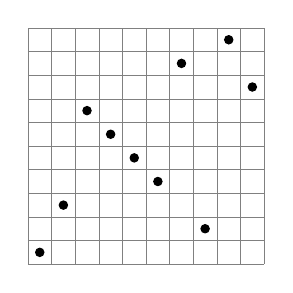
\begin{tikzpicture}[scale=0.3]
    \draw[gray, very thin] (0,0) grid (10,10);

    \filldraw[black] (-0.5+1,-0.5+1) circle (5pt);
    \filldraw[black] (-0.5+2,-0.5+3) circle (5pt);
    \filldraw[black] (-0.5+3,-0.5+7) circle (5pt);
    \filldraw[black] (-0.5+4,-0.5+6) circle (5pt);
    \filldraw[black] (-0.5+5,-0.5+5) circle (5pt);
    \filldraw[black] (-0.5+6,-0.5+4) circle (5pt);
    \filldraw[black] (-0.5+7,-0.5+9) circle (5pt);
    \filldraw[black] (-0.5+8,-0.5+2) circle (5pt);
    \filldraw[black] (-0.5+9,-0.5+10) circle (5pt);
    \filldraw[black] (-0.5+10,-0.5+8) circle (5pt);
  \end{tikzpicture}
  \caption{Sampled uniformly at random from permutations of length $10$. Density of $123$ is $13/40= 0.325$.}
\end{subfigure}\hfill
\begin{subfigure}[t]{0.3\textwidth}
  \centering
  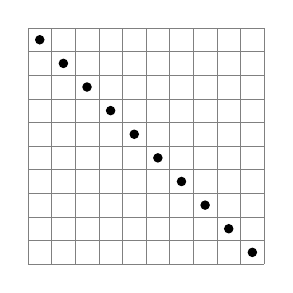
\begin{tikzpicture}[scale=0.3]
    \draw[gray, very thin] (0,0) grid (10,10);
    \foreach \i in {1,...,10}
    {
      \filldraw[black] (-0.5+\i,10.5-\i) circle (5pt);
    }
  \end{tikzpicture}
  \caption{Decreasing permutation. Density of $123$ is $0$.}
\end{subfigure}
\caption{If every triple is a copy of our $123$, the density is $1$. If no triple is a copy of $123$, the density is $0$. There is a spectrum of admissible densities for every pattern, but it does not go all the way to $1$ for almost any of them. What is the highest density in the spectrum for a fixed pattern $\sigma$? We deal with these questions in Part~\ref{part:packing} of the thesis.}
\label{fig:densities_spectrum}
\end{figure}

The question becomes significantly harder when trying to maximise the density of, say, $132$ pattern. As we mention later in Chapter~\ref{chap:packsmall}, a well-known theorem of Erd\H{o}s and Szekeres implies that any permutation of length $n$ (think large) must contain a monotone subpermutation of length at least $\sim \sqrt{n}$, thereby dashing our hopes for the density of $132$ ever being exactly 1 for large $n$ (as some triples will be $123$ and $321$ patterns). This directly motivates the study of questions such as \emph{what is the maximum density of a small pattern $\sigma$ in a permutation of length $n$?} We address these, or questions about the asymptotic versions --- packing densities, in Chapter~\ref{chap:packsmall}.

The purpose of Chapter~\ref{chap:permpack} is to introduce the tool that we developed for our work in Chapter~\ref{chap:packsmall}. The package is called \emph{Permpack} and it automates our search for packing densities of small permutations. 
